%\section{Selection Cuts for eleTau Channel}
\section{\texorpdfstring{Event selection for the \leptonTau channel}{Event selection for the lepton-tau channel}}
\label{sect:eleTauCuts}
Events for the \leptonTau final states (e\Tau and $\mu\Tau$)
were collected with triggers that require 
a loosely isolated \Tau with \PT $>$ 20 \GeV and $|\eta|$ $<$ 2.3 as well as
an isolated electron or muon with $|\eta| < 2.1$.  The minimum
\PT requirement for the electron (muon) was increased during the data taking from 20 to 22 \GeV (17 to 18 \GeV)
due to the increase in instantaneous luminosity.

In the offline analysis the electron, muon, and \Tau objects were required to have \PT $>$ 25, 20, and 25 \GeV, respectively, 
while tightening the corresponding identification and isolation requirements.
In events with more than one opposite-sign \leptonTau pair, we only consider
 the pair that maximizes the scalar sum of \Tau and electron or muon 
transverse momenta.  Events with an additional loosely isolated lepton
with \PT $>$ 10 \GeV are rejected to suppress backgrounds from $Z$ boson
decays.  

Just as for the \Tau\Tau channel we apply preselection requirements to suppress
QCD and \ttbar events, $Z \to \tau \tau$ decays, and low mass resonances.
These requirements are: \mttwo $>$ 40 \GeV, \MPT $>$ 30 GeV, \leptonTau 
invariant mass between 15 and 45 \GeV or $>$ 75 \GeV, $\Delta \Phi > 1$, and we veto events with b-tagged jets.
The final signal region requirements are \mttwo $>$ 90 \GeV and 
\tauMT $>$ 200 \GeV. %where \tauMT is the \Tau transverse mass 
The latter requirement provides discrimination against the \wjets background.  Unlike the \tauTau channel,
events with \mttwo $<$ 90 \GeV are not used because of the higher 
level of background.

%Similar to the \tauTau channel, a hard cut on \mttwo ($>$ 90 \GeV) is useful to suppress different SM backgrounds, especially $W$jets events.
%Such a high cut on the \mttwo increases the sensitivity of the study to signal events with high mass difference. The \Tau transverse mass (\tauMT)
%is found to be a good discriminator to further suppress the $W$jets events which is the main background in this step. 
%Opposite to the \tauTau channel, the events with \mttwo $<$ 90 \GeV are not useful in \leptonTau channels and they can not add any power to 
%the final exclusion. The signal regions for $e\Tau$ and $\mu\Tau$ channels are defined by the following selections:



%\begin{itemize}
%\item \mttwo $>$ 90 \GeV.
%\item \tauMT $>$ 200 \GeV; 
%\end{itemize}

% The composition of the backgrounds and number of remaining signals for both channels can be found in the table \ref{tbl:yieldsLepTau}.

%\begin{table}[!Hhtb]
%\begin{center}
%\begin{tiny}
%\begin{tabular}{lcccccccc}
%\hline
%\hline
%  & SUSY(380,1) & QCD & W & ZX & Top & WW & Higgs & MC \\%& Data \\
%\hline
%\hline
%e\Tau       & 2.14 & 0.0 & 1.29 & 0.38 & 0.02 & 0.05 & 0.06 & 1.79$\pm$0.63 \\%& 3 \\
%\hline
%$\mu\hadtau$& 2.09 & 0.0 & 0.79 & 0.28 & 0.0  & 0.34 & 0.05 & 1.46$\pm$.49 \\%& 5 \\
%QCD 70.87 +- 34.49
%Top 1.15 +- 0.84
%\hline
%\hline
%\end{tabular}
%\caption{MC driven yields for e\Tau and $\mu\hadtau$ channels. Only statistical uncertainties are reported.}
%\label{tbl:yieldsLepTau}
%\end{tiny}
%\end{center}
%\end{table}

Figure \ref{fig:mt2leptontau} % and \ref{fig:taumtleptontau} 
shows the \mttwo distribution after the preselection.
%and the \tauMT distribution after the preselection and the \mttwo requirements, respectively.
The data are in good agreement with the SM expectations. A SUSY signal corresponding to a high mass difference 
 $(m_{\chione}=380\GeV,~m_{\PSGczDo}=1\GeV)$ is used to show the expected signal distribution.

\begin{figure}[!Hhtb]
\centering
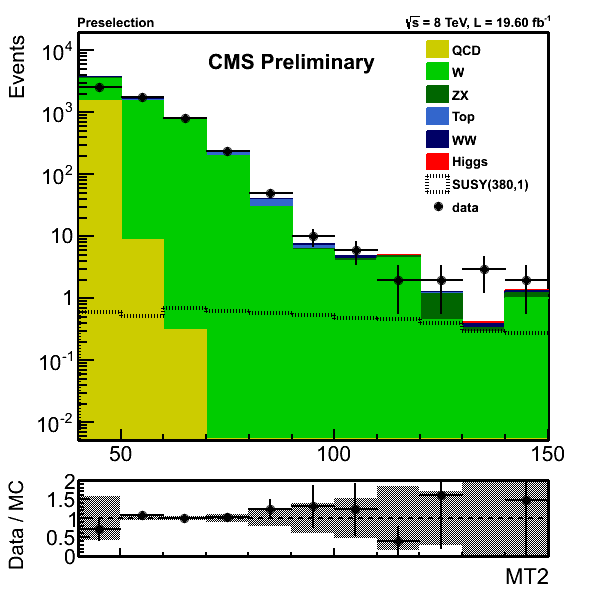
\includegraphics[angle=0,scale=0.35]{SelectionEleTau/MT2.png}
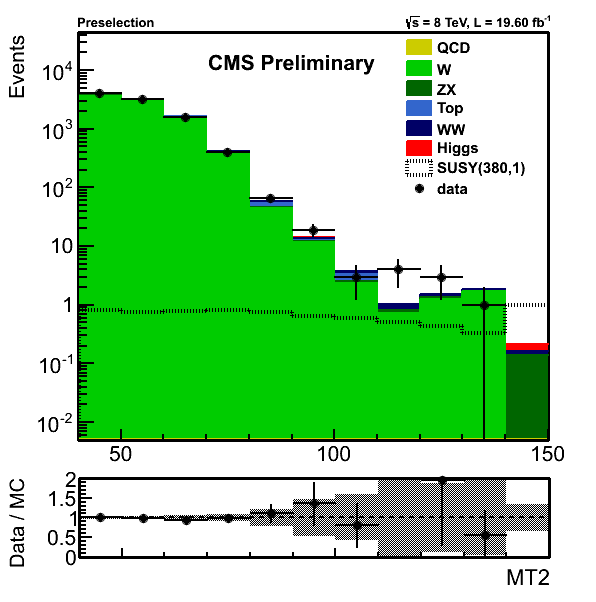
\includegraphics[angle=0,scale=0.35]{SelectionMuTau/MT2_Ratio_Preselection_unBlinded.png}
\caption{\mttwo  distributions for events in the preselection sample, compared to Monte Carlo events in (left) \eTau and (right) \muTau channels. The signal point shown here is $(m_{\chione}=380\GeV,~m_{\PSGczDo}=1\GeV)$.}
\label{fig:mt2leptontau}
\end{figure}


%\begin{figure}[!Hhtb]
%\centering
%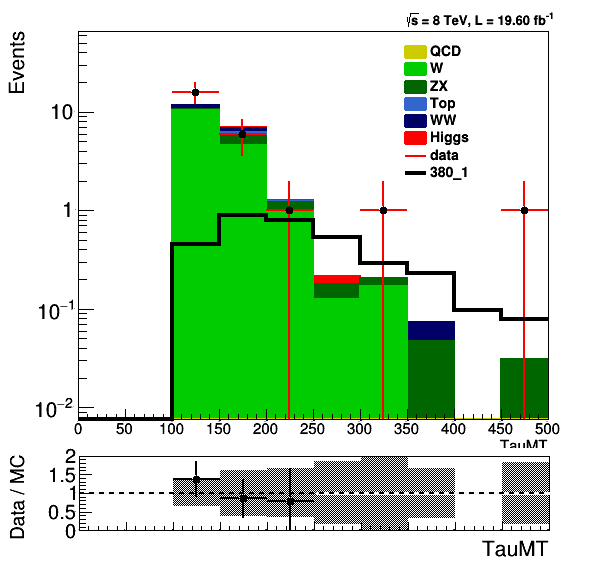
\includegraphics[angle=0,scale=0.35]{SelectionEleTau/TauMT.png}
%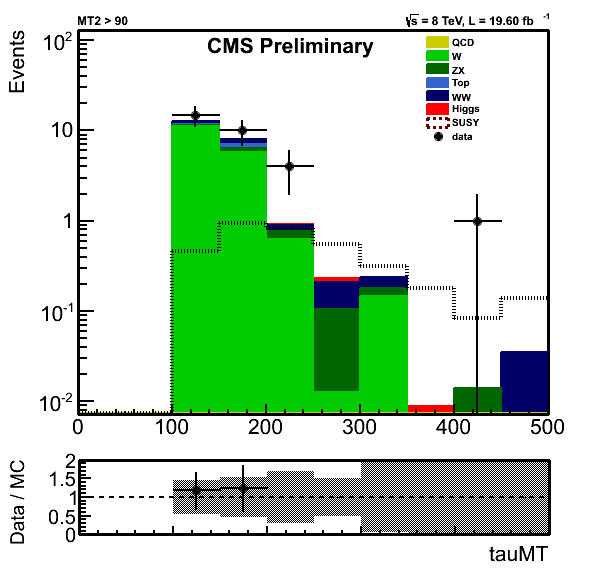
\includegraphics[angle=0,scale=0.35]{SelectionMuTau/tauMT_Ratio_MT2gt90_unBlinded.png}
%\caption{Data-Monte Carlo comparisons of the \tauMT distribution for
%preselected events
%with $\mttwo>$90\GeV in (left) $e\hadtau$ and (right) $\mu\hadtau$ channels.}
%\label{fig:taumtleptontau}
%\end{figure}
%Opposite to the $\Tau\Tau$ channel, the events with $\mttwo<90 \GeV$ are not useful in $\ell\Tau$ channels because of the contamination of
%the Wjets events. It was investigated if increasing the \PT of the objects can increase the sensitivity in this signal region, but no improvement was seen.

